The Silicon Photomultiplier (SiPM), also called Multi-Pixel Photon Counter (MPPC), is a type of photosensor based on silicon developed in the last two decades. SiPMs are replacing progressively conventional PMTs in many experiments and applications. They have outstanding photon counting capabilities at the single photon level with similar gain and higher photodetection efficiency than PMTs. In addition, SiPMs have several advantages as insensitivity to magnetic fields, low operating voltage, compactness and ruggedness. Their main drawback with respect to PMTs is their high dark count rate (between $100~\kilo\hertz$ and $1~\mega\hertz$).

SiPMs are formed by a matrix of Avalanche Photodiodes (APDs) connected in parallel and operating in Geiger mode. APDs, shown in Figure \ref{fig:SchemeAPD}, are based on p-n junctions.
\begin{figure}[htbp]
\centering
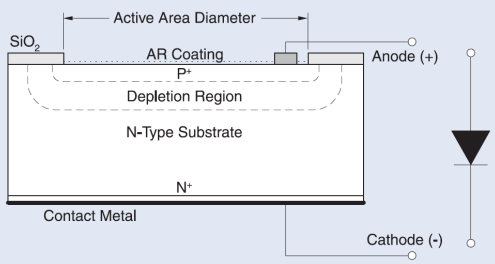
\includegraphics[scale=0.6]{3DesignPrinciples/32Tritium_detector/APD_scheme.png}
\caption{Scheme of an APD and electrical symbol used\label{fig:SchemeAPD}~\cite{OSI}.}
\end{figure}
The voltage $V_ {BD}$ at which a SiPM starts operating in Geiger mode is called the breakdown voltage. At voltages lower than $V_ {BD}$, SiPMs work in the proportional mode in which the signal of each APD is proportional to the energy deposited. The measurement of $V_ {BD}$, described in section \ref{sec:CharacterizationSiPM}, is important to characterize a SiPM since its characteristics depend on the overvoltage $V_{OV}$ defined as the SiPM bias voltage above $V_ {BD}$,
\begin{equation}
V_{OV}=V_{bias}-V_{BD}
\label{overvoltage}
\end{equation}
The SiPM APDs, called pixels, are connected in parallel to give the SiPM output signal. If the photon flux is low enough, each SiPM pixel detects at most one photon. All pixels produce a similar output signal, regardless of the energy deposited. Therefore, the charge of the output signal when $n$ pixels are simultaneously fired is $n$ times the charge of a single pixel. This behaviour is illustrated in Figure \ref{fig:PulsesOfSiPM} where the output signals corresponding to a different number of fired pixels are shown. Hence, the number of detected photons is proportional to the integrated output signal. Once the SiPM is calibrated, the energy of tritium events can be determined. If the photon flux is high (typically several thousands of photons per event) more than one photon impinges simultaneously on the same pixel, producing an output signal corresponding to a single photon. This effect, known as saturation, produces a loss of linearity of the output signal. In the TRITIUM detector, this effect is negligible since tritium electrons produce few photons. %The experimental measurements of this effect, which have been done for our SiPMs, is shown in section \ref{sec:CharacterizationSiPM}. 

\begin{figure}[h]
\centering
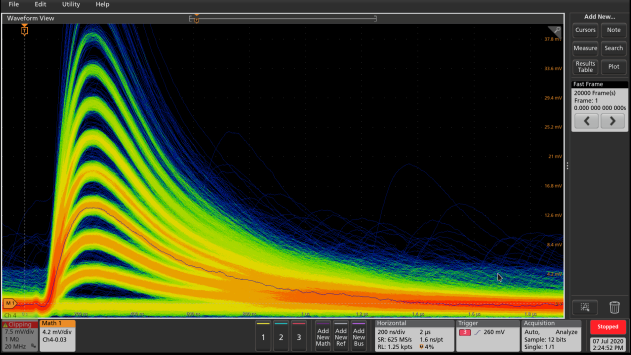
\includegraphics[scale=0.6]{3DesignPrinciples/32Tritium_detector/Several_SiPM_pulses.png}
\caption{SiPM output pulses displayed on the oscilloscope, model MSO44X from Tektronix \cite{Oscilloscope}. Several height pulses are observed, associated to a different number of  SiPM pixels fired at the same time. The persistence function of the oscilloscope is used.\label{fig:PulsesOfSiPM}}
\end{figure}

Different sizes of SiPM pixels are available\footnote{Pixel sizes for commercial SiPMs are $25$, $50$ and $75\mu\meter$ \cite{DataSheetHammamatsu_1_SiPM_25, DataSheetHammamatsu_1_SiPM_50, DataSheetHammamatsu_1_SiPM_75}}. For a given SiPM active area, a small pixel size allows a high dynamic range at the cost of reducing the photon detection efficiency (PDE). As tritium electrons produce few photons, the SiPMs chosen have a large pixel size ($75~\mu\meter$) since we are well within the dynamic range.

%The size of a SiPM pixel should be very small\footnote{Pixel sizes for commercial SiPMs are $25$, $50$ or $75\mu\meter$ \cite{DataSheetHammamatsu_1_SiPM_25}, \cite{DataSheetHammamatsu_1_SiPM_50}, \cite{DataSheetHammamatsu_1_SiPM_75}} to make sure that, for low enough photon fluxes, only one photon is detected in each pixel.

A SiPM can be modelled as an electrical circuit, shown in Figure \ref{subfig:ElectricModelSiPM}. The depletion zone is represented by a capacitance, $C_d$. When a photon impinges on the pixel, the capacitor is discharged, creating an electronic pulse. Each pixel of a SiPM has a quenching resistance\footnote{The typical value of this quenching resistance for commercial SiPMs is around $500~\kilo\Omega$} $R_q$ that limits the avalanche current produced when this pixel is fired. When the discharge is produced, a current flows through the resistance, reducing the reverse voltage seen by the diode. The current through the diode eventually vanishes and the bias voltage is reset. This pixel is ready to detect a new photon. This behaviour is schematically shown in Figure \ref{subfig:HowSiPMworks}. The voltage after photon detection is characteristic of an RC circuit, described by the equation:,
\begin{equation}
V(t)=V_{bias}\left(1-e^{-t/\tau_r} \right)
\label{RCCircuitBiasVoltage}
\end{equation}
where $\tau_r$ is the recovery time constant of the system given by $\tau_r=-C_d R_q$.

\begin{figure}
\centering
    \begin{subfigure}[]{0.45\textwidth}
    \centering
    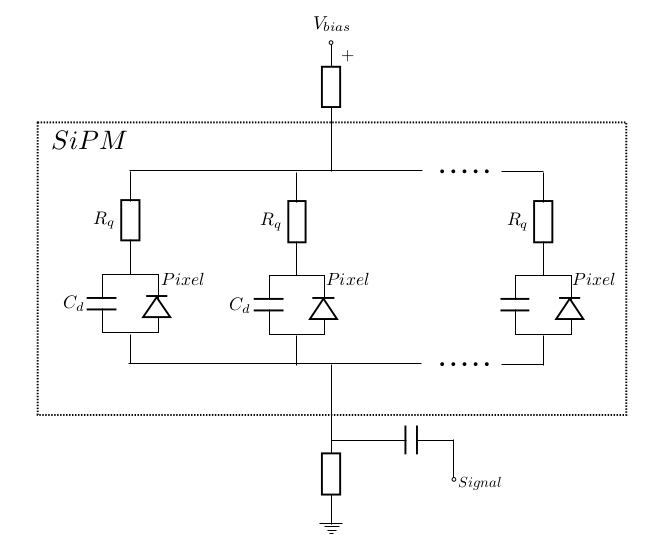
\includegraphics[width=\textwidth]{3DesignPrinciples/32Tritium_detector/SimpliestElectronicSchemeSiPM.png}  
    \caption{\label{subfig:ElectricModelSiPM}}
    \end{subfigure}
    \hfill
    \begin{subfigure}[]{0.45\textwidth}
    \centering
    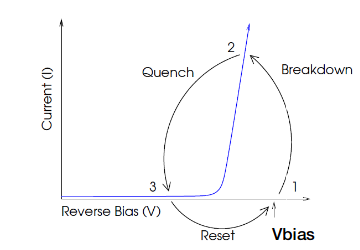
\includegraphics[width=\textwidth]{3DesignPrinciples/32Tritium_detector/How_a_quenching_resistence_in_a_SiPM_works.png}  
    \caption{\label{subfig:HowSiPMworks}}
    \end{subfigure}
 \caption{(a) Electronic scheme of a SiPM and (b) output current of a SiPM as a function of the reverse voltage. As shown, quenching is an essential working mechanism of SiPMs~\cite{DataSheetSensL}.}
 \label{fig:ChenchingResistance}
\end{figure}

The SiPM gain (typically of the order of $10^6$) is defined as the number of e-h pairs produced when a pixel is fired. The gain can be measured from the SiPM single photon spectrum (SPS) which is the spectrum obtained when the SiPM output signal is integrated. The SiPM gain is highly dependent on temperature. As the temperature cannot be controlled with an accuracy better than $1\celsius$ in the final location of the TRITIUM monitor, a gain stabilization method is necessary to compensate for gain variations due to temperature changes.

An important parameter for SiPMs is the PDE, defined as the percentage of the incident photons that are detected. The PDE of a SiPM depends on three different parameters: the fill factor ($FF$), which is the ratio between the active area of the SiPM and its total area, the quantum efficiency ($QE$), which is the probability of producing a photoelectron when a photon hits the SiPM, and the probability $P_{av}$ that an avalanche is produced. Thus, 
\begin{equation}
PDE=FF \times QE \times P_{av}
\label{PDE_SiPM}
\end{equation}
SiPMs produce a dark current that depends on temperature. The dark current and photon events are identical, so they cannot be discriminated. Therefore, it is essential to determine the magnitude of the dark current in the TRITIUM detector.

Avalanche electrons in a pixel can emit secondary optical photons\footnote{Around 20 secondary optical photons are emitted in each pixel for gains of the order of $10^6$ \cite{CrosstalkProbability}}. These optical photons can reach other pixels, producing new avalanches. This effect, called optical cross-talk, produces photoelectrons that add to those truly induced by incident photons, and hence leads to an overestimation of the number of photons detected. The probability of producing an optical crosstalk event depends on the number of electrons produced in the avalanche and, therefore, on temperature and overvoltage. This probability is typically less than $10\%$ at the overvoltage recommended at $25\celsius$ by the manufacturer.

%The PDE, dark count rate and crosstalk are not measured yet since a different setup, shown in reference \cite{PDEStudy}, is needed. These parameters will be measured for the SiPM model used in the final version of TRITIUM monitor.

Due to imperfections existing in the crystal lattice of a SiPM, called traps, an electron of an avalanche can be captured and released after a characteristic time $\tau_a$. If this characteristic time is longer than the pixel recovery time, typically $3\tau$, this electron can trigger a new avalanche which will be seen as a new event. These events, called  afterpulses, are often emitted around $1~\mu\second$ after the incident photon pulses. The afterpulse probability was not measured since it is not relevant for the TRITIUM detector because SiPMs are read out in coincidence within $10~\nano\second$ time. 

The initial SiPM candidate for the TRITIUM detector and the one which was characterized in this thesis is the model S13360-1375 from Hamamatsu Photonics \cite{DataSheetHammamatsu_1_SiPM_1375} whose characteristics are given in Table \ref{tab:PropertiesOfSiPM1375}. This model was mainly chosen due to its large pixel size, $75~\mu\meter$, which implies high PDE and gain. This SiPM model was later replaced by the model S13360-6075 from Hamamatsu Photonics \cite{DataSheetHammamatsu_1_SiPM_75}, whose characteristics are also listed in Table \ref{tab:PropertiesOfSiPM1375}. The only difference between this model and the first is its larger active area ($6\times6~\mm^2$) that allows reading more scintillating fibres but at the price of a higher dark count rate (typically 2 Mcps).
\begin{table}[htbp]
\centering{}%
\begin{tabular}{lcc}
\toprule 
Characteristics & S13360-1375 & S13360-6075 \tabularnewline
\midrule
\midrule 
Series & $S13360$ & $S13360$ \tabularnewline
Model & $1375$ & $6075$ \tabularnewline
Pixel Pitch ($\mu\meter$) & $75$ & $75$ \tabularnewline
Effective photosensitive area ($\mm^2$) & $1.3 \times 1.3$ & $6.0 \times 6.0$ \tabularnewline
Number of pixels & $285$ & $6400$ \tabularnewline
Fill factor & $82\%$ & $82\%$ \tabularnewline
Refractive index of windows material & $1.55$ & $1.55$ \tabularnewline
Operating temperature range ($\celsius$) & $[-20,60]$ & $[-20,60]$ \tabularnewline
Spectral response range, $\lambda$ ($\nano\meter$) & $[320, 900]$ & $[320, 900]$ \tabularnewline
Peak sensitivity wavelength, $\lambda_p$ ($\nano\meter$) & $450$ & $450$ \tabularnewline
PDE ($\%$) & $50$ & $50$ \tabularnewline
Dark counts, Typical/Maximum (kcps) & $90/270$ & $2000/6000$ \tabularnewline
Terminal capacitance, $C_t$ ($\pico\farad$) & $60$ & $1280$ \tabularnewline
Gain & $4 \cdot{} 10^6$ & $4 \cdot{} 10^6$ \tabularnewline
$V_{BD}$ ($\volt$) & $50.97$ & $53$ \tabularnewline
Cross talk probability($\%$) & $7$ & $7$ \tabularnewline
Temperature coefficient (m$\volt/\celsius$) & $54$ & $54$ \tabularnewline
\bottomrule
\end{tabular}
\caption{Characteristics of SiPM S13360-1375 and S13360-6075 from Hamamatsu Photonics \cite{DataSheetHammamatsu_1_SiPM_1375}.}
\label{tab:PropertiesOfSiPM1375}
\end{table}
The parameters quoted in Table \ref{tab:PropertiesOfSiPM1375}, are typical values provided by the manufacturer. They can vary from one SiPM to another of the same model. Thus, it is necessary to measure them. Some of these measurements are reported in section \ref{sec:CharacterizationSiPM}.  This SiPM was also chosen because its maximum PDE is reached at $\lambda_{p,SiPM}=450~\nano\meter$, as can be observed in Figure \ref{fig:PDESiPM}. This wavelength is very close to the peak of the emission spectrum of the scintillating fibres used, $\lambda_{p,fibre}=435~\nano\meter$.
\begin{figure}[htbp]
\centering
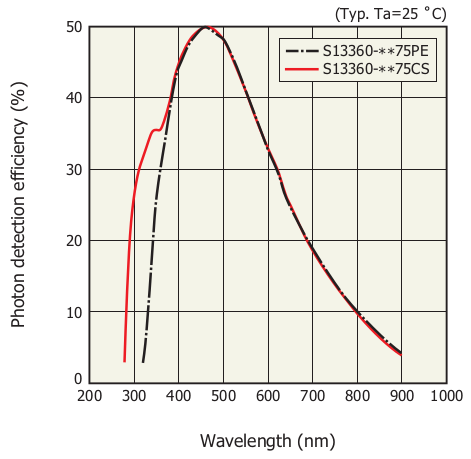
\includegraphics[scale=0.6]{3DesignPrinciples/32Tritium_detector/SiPMPDE.png}
\caption{PDE spectrum for SiPM S13360-**75 models~\cite{DataSheetHammamatsu_1_SiPM_1375}.\label{fig:PDESiPM}}
\end{figure}
The characteristics was carried out at the level of a single SiPM to measure its characteristics and to test the gain control method. %A new experimental setup, detailed in appendix \ref{App:ElectronicReadoutSiPM}, is already  prepared to perform a complete characterization of the SiPM model S13360-6075.